\documentclass[journal,12pt,twocolumn]{IEEEtran}
\usepackage{setspace}
\usepackage{gensymb}
\usepackage{caption}
%\usepackage{multirow}
%\usepackage{multicolumn}
%\usepackage{subcaption}
%\doublespacing
\singlespacing
\usepackage{csvsimple}
\usepackage{amsmath}
\usepackage{multicol}
\usepackage{enumerate}
\usepackage{amssymb}
\usepackage{graphicx}
\usepackage{newfloat}
\usepackage{float}
%\usepackage{syntax}
\usepackage{listings}
%\usepackage{iithtlc}
\usepackage{color}
\usepackage{tikz}
\usetikzlibrary{shapes,arrows}
\usepackage{relsize}


%\usepackage{graphicx}
%\usepackage{amssymb}
%\usepackage{relsize}
%\usepackage[cmex10]{amsmath}
%\usepackage{mathtools}
%\usepackage{amsthm}
%\interdisplaylinepenalty=2500
%\savesymbol{iint}
%\usepackage{txfonts}
%\restoresymbol{TXF}{iint}
%\usepackage{wasysym}
\usepackage{amsthm}
\usepackage{mathrsfs}
\usepackage{txfonts}
\usepackage{stfloats}
\usepackage{cite}
\usepackage{cases}
\usepackage{mathtools}
\usepackage{caption}
\usepackage{enumerate}	
\usepackage{enumitem}
\usepackage{amsmath}
%\usepackage{xtab}
\usepackage{longtable}
\usepackage{multirow}
%\usepackage{algorithm}
%\usepackage{algpseudocode}
\usepackage{enumitem}
\usepackage{mathtools}
\usepackage{hyperref}
%\usepackage[framemethod=tikz]{mdframed}
\usepackage{listings}
    %\usepackage[latin1]{inputenc}                                 %%
    \usepackage{color}                                            %%
    \usepackage{array}                                            %%
    \usepackage{longtable}                                        %%
    \usepackage{calc}                                             %%
    \usepackage{multirow}                                         %%
    \usepackage{hhline}                                           %%
    \usepackage{ifthen}                                           %%
  %optionally (for landscape tables embedded in another document): %%
    \usepackage{lscape}     


\usepackage{url}
\def\UrlBreaks{\do\/\do-}


%\usepackage{stmaryrd}


%\usepackage{wasysym}
%\newcounter{MYtempeqncnt}
\DeclareMathOperator*{\Res}{Res}
%\renewcommand{\baselinestretch}{2}
\renewcommand\thesection{\arabic{section}}
\renewcommand\thesubsection{\thesection.\arabic{subsection}}
\renewcommand\thesubsubsection{\thesubsection.\arabic{subsubsection}}

\renewcommand\thesectiondis{\arabic{section}}
\renewcommand\thesubsectiondis{\thesectiondis.\arabic{subsection}}
\renewcommand\thesubsubsectiondis{\thesubsectiondis.\arabic{subsubsection}}

% correct bad hyphenation here
\hyphenation{op-tical net-works semi-conduc-tor}

%\lstset{
%language=C,
%frame=single, 
%breaklines=true
%}

%\lstset{
	%%basicstyle=\small\ttfamily\bfseries,
	%%numberstyle=\small\ttfamily,
	%language=Octave,
	%backgroundcolor=\color{white},
	%%frame=single,
	%%keywordstyle=\bfseries,
	%%breaklines=true,
	%%showstringspaces=false,
	%%xleftmargin=-10mm,
	%%aboveskip=-1mm,
	%%belowskip=0mm
%}

%\surroundwithmdframed[width=\columnwidth]{lstlisting}
\def\inputGnumericTable{}                                 %%
\lstset{
%language=C,
frame=single, 
breaklines=true,
columns=fullflexible
}
 

\begin{document}
\tikzstyle{block} = [rectangle, draw,
    text width=3em, text centered, minimum height=3em]
\tikzstyle{sum} = [draw, circle, node distance=3cm]
\tikzstyle{input} = [coordinate]
\tikzstyle{output} = [coordinate]
\tikzstyle{pinstyle} = [pin edge={to-,thin,black}]

\theoremstyle{definition}
\newtheorem{theorem}{Theorem}[section]
\newtheorem{problem}{Problem}
\newtheorem{proposition}{Proposition}[section]
\newtheorem{lemma}{Lemma}[section]
\newtheorem{corollary}[theorem]{Corollary}
\newtheorem{example}{Example}[section]
\newtheorem{definition}{Definition}[section]
%\newtheorem{algorithm}{Algorithm}[section]
%\newtheorem{cor}{Corollary}
\newcommand{\BEQA}{\begin{eqnarray}}
\newcommand{\EEQA}{\end{eqnarray}}
\newcommand{\define}{\stackrel{\triangle}{=}}
\bibliographystyle{IEEEtran}
%\bibliographystyle{ieeetr}
\providecommand{\nCr}[2]{\,^{#1}C_{#2}} % nCr
\providecommand{\nPr}[2]{\,^{#1}P_{#2}} % nPr
\providecommand{\mbf}{\mathbf}
\providecommand{\pr}[1]{\ensuremath{\Pr\left(#1\right)}}
\providecommand{\qfunc}[1]{\ensuremath{Q\left(#1\right)}}
\providecommand{\sbrak}[1]{\ensuremath{{}\left[#1\right]}}
\providecommand{\lsbrak}[1]{\ensuremath{{}\left[#1\right.}}
\providecommand{\rsbrak}[1]{\ensuremath{{}\left.#1\right]}}
\providecommand{\brak}[1]{\ensuremath{\left(#1\right)}}
\providecommand{\lbrak}[1]{\ensuremath{\left(#1\right.}}
\providecommand{\rbrak}[1]{\ensuremath{\left.#1\right)}}
\providecommand{\cbrak}[1]{\ensuremath{\left\{#1\right\}}}
\providecommand{\lcbrak}[1]{\ensuremath{\left\{#1\right.}}
\providecommand{\rcbrak}[1]{\ensuremath{\left.#1\right\}}}
\theoremstyle{remark}
\newtheorem{rem}{Remark}
\newcommand{\sgn}{\mathop{\mathrm{sgn}}}
%\providecommand{\abs}[1]{\left\vert#1\right\vert}
\providecommand{\res}[1]{\Res\displaylimits_{#1}} 
%\providecommand{\norm}[1]{\left\Vert#1\right\Vert}
\providecommand{\mtx}[1]{\mathbf{#1}}
%\providecommand{\mean}[1]{E\left[ #1 \right]}
\providecommand{\fourier}{\overset{\mathcal{F}}{ \rightleftharpoons}}
%\providecommand{\hilbert}{\overset{\mathcal{H}}{ \rightleftharpoons}}
\providecommand{\system}{\overset{\mathcal{H}}{ \longleftrightarrow}}
	%\newcommand{\solution}[2]{\textbf{Solution:}{#1}}
\newcommand{\solution}{\noindent \textbf{Solution: }}
\newcommand{\myvec}[1]{\ensuremath{\begin{pmatrix}#1\end{pmatrix}}}
\providecommand{\dec}[2]{\ensuremath{\overset{#1}{\underset{#2}{\gtrless}}}}
\DeclarePairedDelimiter{\ceil}{\lceil}{\rceil}
%\numberwithin{equation}{section}
%\numberwithin{problem}{subsection}
%\numberwithin{definition}{subsection}
\makeatletter
\@addtoreset{figure}{section}
\makeatother
\let\StandardTheFigure\thefigure
%\renewcommand{\thefigure}{\theproblem.\arabic{figure}}
\renewcommand{\thefigure}{\thesection}
%\numberwithin{figure}{subsection}
%\numberwithin{equation}{subsection}
%\numberwithin{equation}{section}
%\numberwithin{equation}{problem}
%\numberwithin{problem}{subsection}
\numberwithin{problem}{section}
%%\numberwithin{definition}{subsection}
%\makeatletter
%\@addtoreset{figure}{problem}
%\makeatother
\makeatletter
\@addtoreset{table}{section}
\makeatother
\let\StandardTheFigure\thefigure
\let\StandardTheTable\thetable
\let\vec\mathbf
\numberwithin{equation}{section}
\vspace{3cm}

\title{%Convex Optimization in Python
	\logo{
	Random Numbers
	}
}
%\title{
%	\logo{Matrix Analysis through Octave}{\begin{center}\includegraphics[scale=.24]{tlc}\end{center}}{}{HAMDSP}
%}
% paper title
% can use linebreaks \\ within to get better formatting as desired
%\title{Matrix Analysis through Octave}
%
%
% author names and IEEE memberships
% note positions of commas and nonbreaking spaces ( ~ ) LaTeX will not break
% a structure at a ~ so this keeps an author's name from being broken across
% two lines.
% use \thanks{} to gain access to the first footnote area
% a separate \thanks must be used for each paragraph as LaTeX2e's \thanks
% was not built to handle multiple paragraphs
%
\author{Bandaru Naresh Kumar% <-this % stops a space
% <-this % stops a space
%\thanks{J. Doe and J. Doe are with Anonymous University.}% <-this % stops a space
%\thanks{Manuscript received April 19, 2005; revised January 11, 2007.}}
}
% note the % following the last \IEEEmembership and also \thanks - 
% these prevent an unwanted space from occurring between the last author name
% and the end of the author line. i.e., if you had this:
% 
% \author{....lastname \thanks{...} \thanks{...} }
%                     ^------------^------------^----Do not want these spaces!
%
% a space would be appended to the last name and could cause every name on that
% line to be shifted left slightly. This is one of those "LaTeX things". For
% instance, "\textbf{A} \textbf{B}" will typeset as "A B" not "AB". To get
% "AB" then you have to do: "\textbf{A}\textbf{B}"
% \thanks is no different in this regard, so shield the last } of each \thanks
% that ends a line with a % and do not let a space in before the next \thanks.
% Spaces after \IEEEmembership other than the last one are OK (and needed) as
% you are supposed to have spaces between the names. For what it is worth,
% this is a minor point as most people would not even notice if the said evil
% space somehow managed to creep in.
% The paper headers
%\markboth{Journal of \LaTeX\ Class Files,~Vol.~6, No.~1, January~2007}%
%{Shell \MakeLowercase{\textit{et al.}}: Bare Demo of IEEEtran.cls for Journals}
% The only time the second header will appear is for the odd numbered pages
% after the title page when using the twoside option.
% 
% *** Note that you probably will NOT want to include the author's ***
% *** name in the headers of peer review papers.                   ***
% You can use \ifCLASSOPTIONpeerreview for conditional compilation here if
% you desire.
% If you want to put a publisher's ID mark on the page you can do it like
% this:
%\IEEEpubid{0000--0000/00\$00.00~\copyright~2007 IEEE}
% Remember, if you use this you must call \IEEEpubidadjcol in the second
% column for its text to clear the IEEEpubid mark.
% make the title area

\maketitle
\tableofcontents
\bigskip
\renewcommand{\thefigure}{\theenumi}
\renewcommand{\thetable}{\theenumi}
%%
\section{Uniform Random Numbers}
Let $U$ be a uniform random variable between 0 and 1.
\begin{enumerate}[label=\thesection.\arabic*
,ref=\thesection.\theenumi]
\item Generate $10^6$ samples of $U$ using a C program and save into a file called uni.dat .
\\
\solution Download the following files and execute the  C program.
\begin{lstlisting}
wget https://github.com/NareshBandaru13/Random-Numbers/blob/main/ex1/1/exrand.c
wget https://github.com/NareshBandaru13/Random-Numbers/blob/main/ex1/1/coeffs.h
\end{lstlisting}
Use the below command in the terminal to run the code
\begin{lstlisting}
gcc exrand.c -lm
./a.out
\end{lstlisting}

%
\item
Load the uni.dat file into python and plot the empirical CDF of $U$ using the samples in uni.dat. The CDF is defined as
\begin{align}
F_{U}(x) = \pr{U \le x}
\end{align}
\\
\solution 
The graph \ref{fig:uni_cdf} is obtained by running the below code
\begin{lstlisting}
https://github.com/NareshBandaru13/Random-Numbers/blob/main/ex1/2/main.py
\end{lstlisting}
Run the following command in the terminal to run the code.\\
\begin{lstlisting}
python3 main.py
\end{lstlisting}

\begin{figure}[H]
\centering
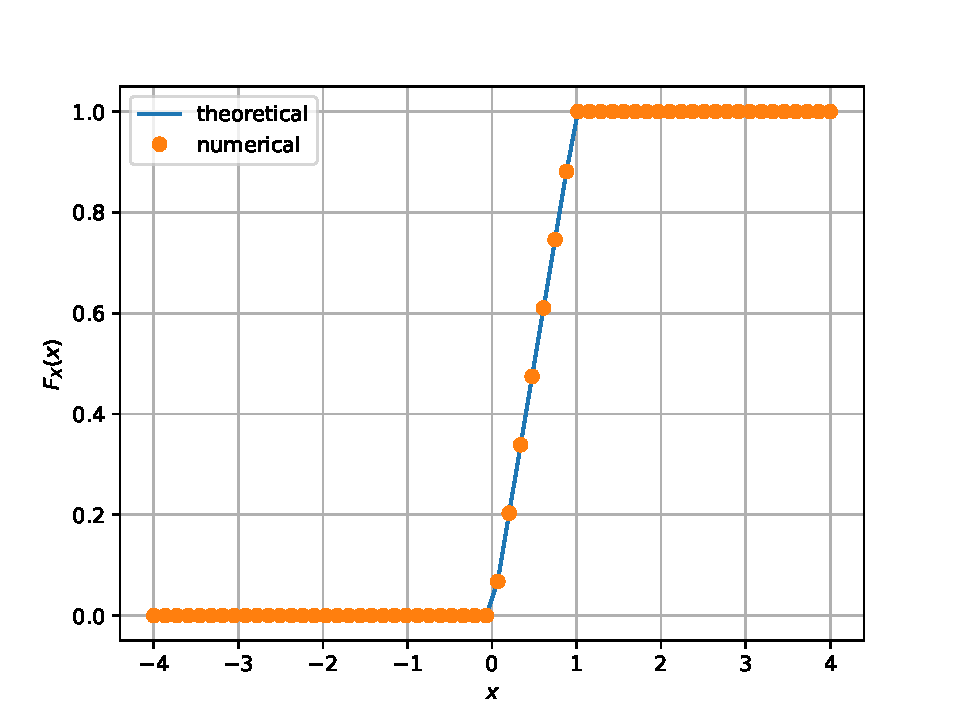
\includegraphics[width=\columnwidth]{uni_cdf.pdf}
\caption{The CDF of $U$}
\label{fig:uni_cdf}
\end{figure}
%
\item
Find a  theoretical expression for $F_{U}(x)$.\\
\solution
Given U is uniform random variable so
\[
  f_X (x) =
 \begin{cases}
 1  & 0 \le x \le 1 \\
 0  & otherwise \\
 \end{cases}
\]
\begin{align*}
    F_X (x) &= \int_{-\infty} ^{x} f_X (x) dx \\
          &= 0 + \int_{0} ^{x} 1 dx \\
          &= 
\begin{cases}
 1 & x >1 \\
 x & 0 \le x \le 1 \\
 0  & x<0 \\
 \end{cases}
\end{align*}	
\item
The mean of $U$ is defined as
%
\begin{equation}
E\sbrak{U} = \frac{1}{N}\sum_{i=1}^{N}U_i
\end{equation}
%
and its variance as
%
\begin{equation}
\text{var}\sbrak{U} = E\sbrak{U- E\sbrak{U}}^2 
\end{equation}
Write a C program to  find the mean and variance of $U$. \\
\solution
\begin{lstlisting}
wget https://github.com/NareshBandaru13/Random-Numbers/blob/main/ex1/4/exrand.c
wget https://github.com/NareshBandaru13/Random-Numbers/blob/main/ex1/4/coeffs.h 
\end{lstlisting}
Use below command to run file,
\begin{lstlisting}
gcc exrand.c -lm
./a.out
\end{lstlisting}
\item Verify your result theoretically given that
$$E[U^{k}] = \int_{-\infty} ^{\infty} x^{k}dF_X (x)$$
\end{enumerate}
%
Given
$$E[U^{k}] = \int_{-\infty} ^{\infty} x^{k}dF_X (x)$$
     \begin{align*}
        E[U] &= \int_{-\infty} ^{\infty} x^{k}f_X (x) dx \\
           &= \int_{0} ^{1} x \times 1 dx \\
           &= \left[\frac{x^2}{2}\right]_{0} ^{1} = \frac{1}{2}
     \end{align*} 
if k=2 
       \begin{align*}
          E[U^2] &= \int_{0} ^{1} x^{2}\times 1 dx \\
          &= \left[\frac{x^3}{3}\right]_{0} ^{1} = \frac{1}{3}
          \end{align*}\\
      \begin{align*}
    variance &= E[u-E[u]]^{2} \\
    &= E[U^{2}]-E^{2}[U] \\
    &= \frac{1}{3} - \frac{1}{4} = 0.0833 \\
     \end{align*}
    
\section{Central Limit Theorem}
\begin{enumerate}[label=\thesection.\arabic*,ref=\thesection.\theenumi]

\item
Generate $10^6$ samples of the random variable
%
\begin{equation}
X = \sum_{i=1}^{12}U_i -6
\end{equation}
%
using a C program, where $U_i, i = 1,2,\dots, 12$ are  a set of independent uniform random variables between 0 and 1
and save in a file called gau.dat
\\
\solution
\begin{lstlisting}
wget https://github.com/NareshBandaru13/Random-Numbers/blob/main/ex2/1/exrand.c
wget https://github.com/NareshBandaru13/Random-Numbers/blob/main/ex2/1/coeffs.h
\end{lstlisting}
Running the above codes generates uni.dat and gau.dat file.
Use the command 
\begin{lstlisting}
gcc exrand.c -lm
.\a.out
\end{lstlisting}

\item
Load gau.dat in python and plot the empirical CDF of $X$ using the samples in gau.dat. What properties does a CDF have?
\\
\solution 
The CDF of $X$ is plotted in plot,Properties of the CDF:
\begin{itemize}
\item $F_X (x)=P(X \leq x) $
\item $Q_X (x) = P(X > x)$
\item  $F_X (x) = 1 - Q_X (x)$ This can be used to calculate F (x).
\end{itemize}

\begin{figure}[H]
\centering
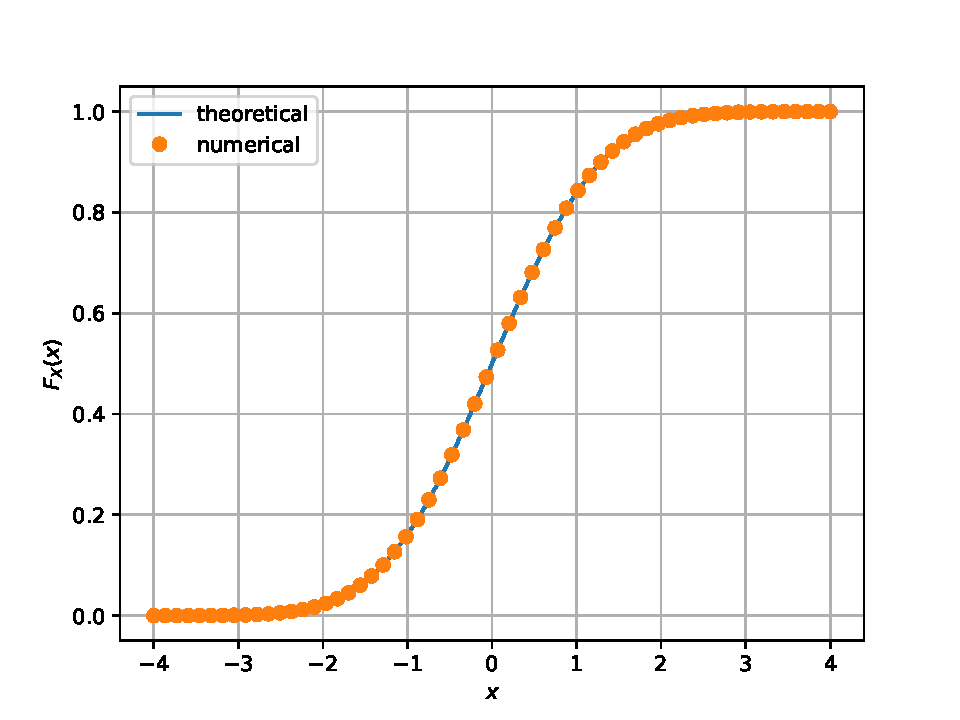
\includegraphics[width=\columnwidth]{gau_cdf.pdf}
\caption{The CDF of $X$}
\label{fig:gau_cdf}
\end{figure}

\item
Load gau.dat in python and plot the empirical PDF of $X$ using the samples in gau.dat. The PDF of $X$ is defined as
\begin{align}
p_{X}(x) = \frac{d}{dx}F_{X}(x)
\end{align}
What properties does the PDF have?
\\
\begin{figure}[H]
\centering
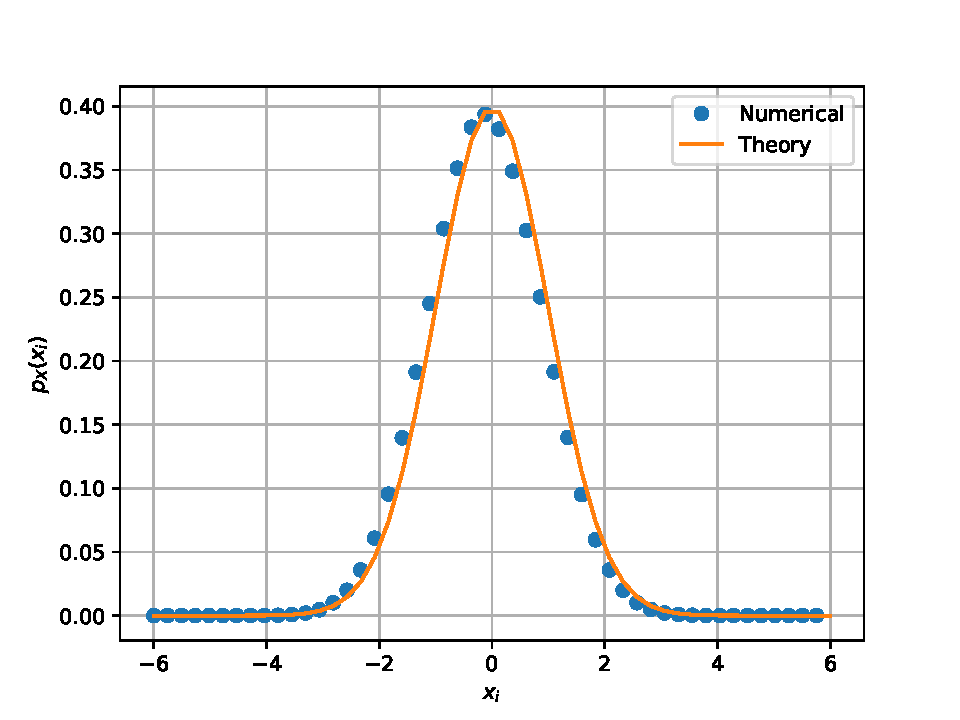
\includegraphics[width=\columnwidth]{gauss_pdf.pdf}
\caption{The PDF of $X$}
\label{fig:gauss_pdf}
\end{figure}

\solution The PDF of $X$ is plotted  using the code below
\begin{lstlisting}
https://github.com/NareshBandaru13/Random-Numbers/blob/main/ex2/3/main.py
\end{lstlisting}
Use the below command to run the code:
\begin{lstlisting}
python3 main.py
\end{lstlisting}
Properties of PDF:
\begin{itemize}
\item PDF is symmetric about $x \approx 0$\\
\item graph is similar to bell shaped\\
\item mean of graph is situated at the symmetrical point\\
\end{itemize}

\item Find the mean and variance of $X$ by writing a C program.\\
\solution
Running the below code gives \\
Mean = 0.000326
Variance= 1.000906
 \begin{lstlisting}
https://github.com/NareshBandaru13/Random-Numbers/blob/main/ex2/4/exrand.c
\end{lstlisting}
Command used:
\begin{lstlisting}
gcc exrand.c -lm
./a.out
\end{lstlisting}

\item Given that 
$$p_X (x) = \frac{1}{\sqrt{2\pi}}e^{-\frac{x^2}{2}} ,-\infty <x< \infty$$
by property of probability $$\int_{-\infty} ^{\infty} p_X (x)dx = 1$$
\begin{align*}
    F_X (x) &= \int_{-\infty} ^{x} p_X (x) dx\\
     &=  \int_{-\infty} ^{x} \frac{1}{\sqrt{2\pi}}e^{-\frac{x^2}{2}} \\
\end{align*}

\begin{align*}
    E[X] &= \int_{-\infty} ^{\infty} xp(x) dx \\
    &= \int_{-\infty} ^{\infty} \frac{x}{\sqrt{2\pi}} e^{\frac{-x^2}{2}}dx \\
\end{align*}
$\frac{x}{\sqrt{2\pi}} e^{\frac{-x^2}{2}}$ is an odd function so integral is zero i.e $E[X] = 0$. \\

\begin{align*}
    E[X^2] &= \int_{-\infty}  ^{\infty} x^{2} p(x) dx \\
    &= x\int_{-\infty} ^{\infty} xp(x) dx - \int_{-\infty} ^{\infty} \left(\int xp(x) dx\right)dx\\
    &= \left[-x\frac{1}{\sqrt{2\pi}}e^{\frac{-x^2}{2}}\right]_{-\infty} ^{\infty} - \int_{-\infty} ^{\infty} -\frac{1}{\sqrt{2\pi}}e^{\frac{-x^2}{2}} dx  \\
    &= 0 - (-1)
    &= 1
\end{align*}
we know that
$$\int_{-\infty} ^{\infty} e^{-\frac{x^2}{2}} = \sqrt{2\pi}$$
by series expansion $\frac{x}{e^{\frac{x^2}{2}}} = \frac{x}{1 +\frac{x^2}{2} + \frac{x^4}{8} + ... }$ \\
putting $x = \infty$,we get $\frac{1}{\infty} = 0$ \\
Similarly when $x = -\infty$ we get 0 \\
$var(x) = E[x^2] - E[x] = 1 - 0 =1$
\end{enumerate}

\section{From Uniform to Other}
\begin{enumerate}[label=\thesection.\arabic*,ref=\thesection.\theenumi]
\item
Generate samples of 
%
\begin{equation}
V = -2\ln\brak{1-U}
\end{equation}
%
and plot its CDF.\\ 
\solution

Running the below code generates samples of V from file uni.dat(U).
\begin{lstlisting}
https://github.com/NareshBandaru13/Random-Numbers/blob/main/ex3/main.py
\end{lstlisting}
Use the below command in the terminal to run the code:
\begin{lstlisting}
python3 main.py
\end{lstlisting}
Now these samples are used to plot  by running the below code
 \begin{figure}[H]
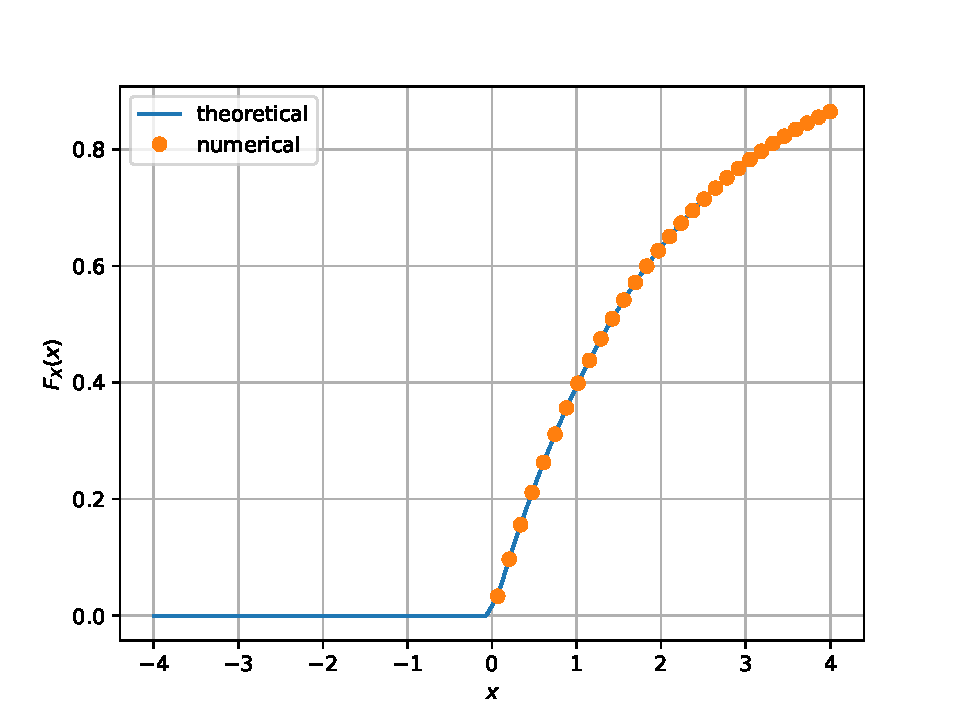
\includegraphics[width=0.5\textwidth]{V_cdf.pdf}
\caption{CDF for (3)}
\label{fig:V}
\end{figure}
\begin{lstlisting}
https://github.com/NareshBandaru13/Random-Numbers/blob/main/ex3/cdf.py
\end{lstlisting}
Use the below command to run the code:
\begin{lstlisting}
python3 cdf.py
\end{lstlisting}

\item
Theorotical expression for $F_V (x)$
\begin{align*}
    F_V (x) &= P\{V \le x\} \\
            &= P\{-2\times \ln{(1-U)} \le x\} \\
            &= P\{U \le 1 - e^{(-\frac{x}{2})}\} \\ 
            &= F_U\{1- e^{(-\frac{x}{2})} \}\\
            &=
\begin{cases}
 1 - e^{(-\frac{x}{2})} & 0 \le x < \infty \\
 0  & x<0 \\
 \end{cases}
\end{align*} 
\end{enumerate}

\section{Triangular Distribution}
\begin{enumerate}[label=\thesection.\arabic*
,ref=\thesection.\theenumi]
%
\item Generate 
	\begin{align}
		T = U_1+U_2
	\end{align}
we get the code
\begin{lstlisting}
https://github.com/NareshBandaru13/Random-Numbers/blob/main/ex4/1/main.py
\end{lstlisting}
run the command
\begin{lstlisting}
python3 main.py
\end{lstlisting}

\item Find the CDF of $T$.
we have code
\begin{lstlisting}
https://github.com/NareshBandaru13/Random-Numbers/blob/main/ex4/2/main1.py
\end{lstlisting}
run the command
\begin{lstlisting}
python3 main1.py
\end{lstlisting}
\begin{figure}[H]
    \centering
    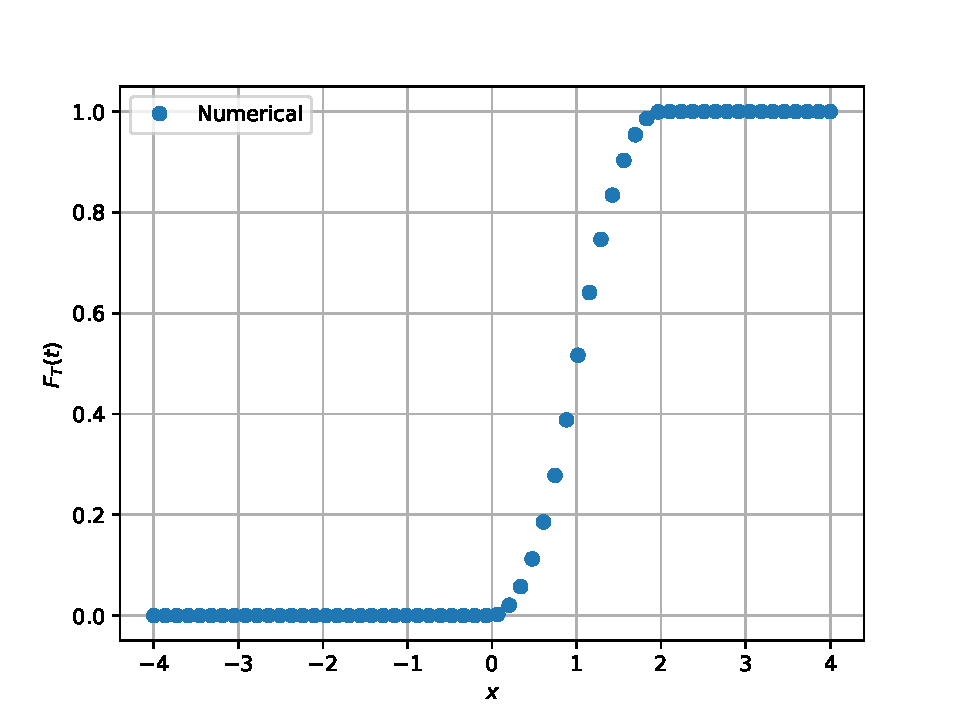
\includegraphics[scale = 0.5]{t1.pdf}
    \caption{numerical cdf}
    \label{fig:my_cdf1}
\end{figure}

\item Find the PDF of $T$
we have code
\begin{lstlisting}
https://github.com/NareshBandaru13/Random-Numbers/blob/main/ex4/3/main2.py
\end{lstlisting}
run the command
\begin{lstlisting}
python3 main2.py
\end{lstlisting}

\begin{figure}[H]
    \centering
    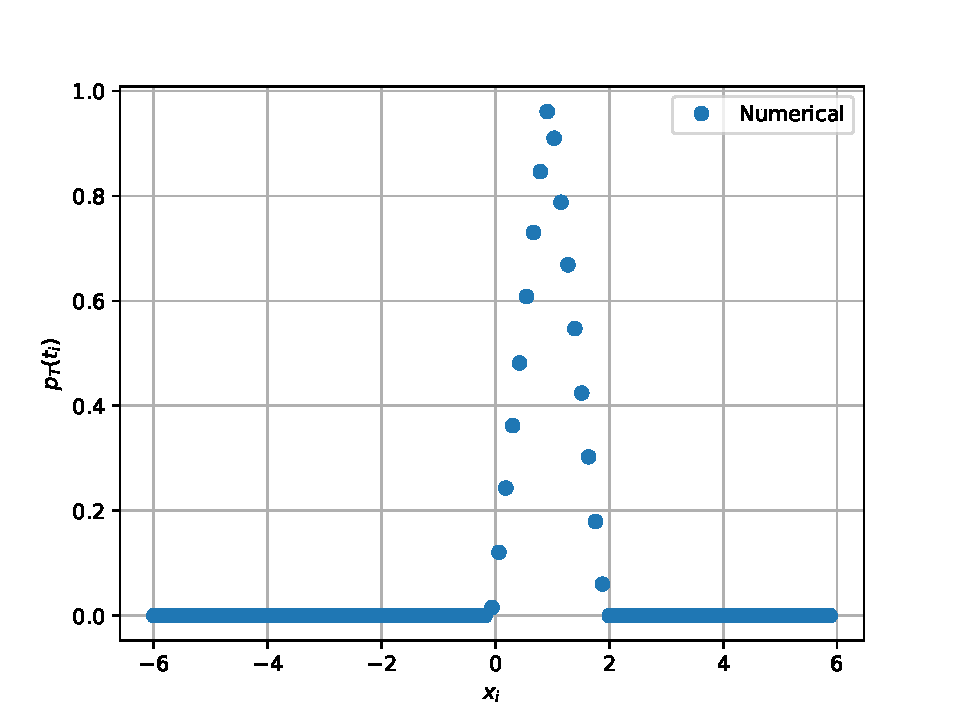
\includegraphics[scale = 0.5]{t2.pdf}
    \caption{Numerical cdf}
    \label{fig:my_cdf2}
\end{figure}

\item Find the theoretical expressions for the PDF and CDF of $T$.
\solution

  \begin{align*}
      F_T (t) &= P\{T \le t\} \\
       &= P\{ U1 + U2 \le t\} \\
  \end{align*}
let us take two cases if $0 \le t \le 1$ and
$1 < t \le 2$ \\
\begin{figure}[H]
    \centering
    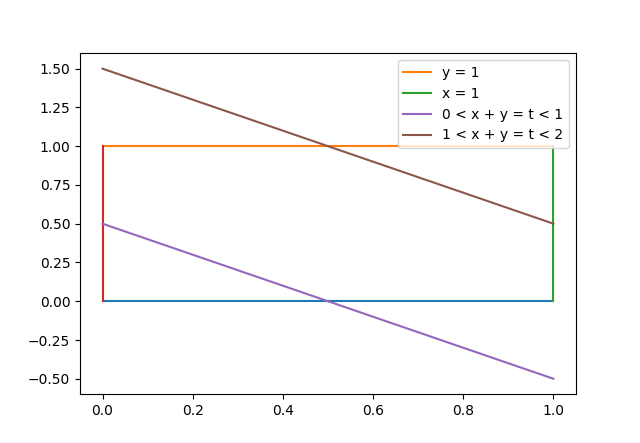
\includegraphics[scale = 0.6]{cdf.png}
    \caption{def plot}
    \label{fig:my_defplot}
\end{figure}
The above graph is produced by
\begin{lstlisting}
https://github.com/NareshBandaru13/Random-Numbers/blob/main/ex4/2/find.py
\end{lstlisting}
Run the code in terminal
\begin{lstlisting}
python3 find.py
\end{lstlisting}
from the figures it is evident that
$P(U1+U2 < t ,0\le t <1) = \frac{t^2}{2}$ \\
$P(U1+U2 < t ,1\le t \le2) =1 - \frac{(2 -t)^2}{2}$ \\
\[
F_T (t) = 
\begin{cases}
0 & t<0\\
\frac{t^2}{2} & 0\leq t \leq 1\\
1-\frac{(2-t)^{2}}{2} & 1< t \leq 2\\
1 & t>2
\end{cases}
\]
\begin{align*}
P_{T}(t)=\frac{d(F_{T}(t))}{dt}\\
\therefore P_{T}(t)=
\begin{cases}
0 & t<0\\
t & 0\leq t \leq 1\\
2-t  & 0< t \leq 2\\
0 & t>2 
\end{cases}    
\end{align*}

\item Verify your results through a plot
Take the code for cdf
\begin{lstlisting}
https://github.com/NareshBandaru13/Random-Numbers/blob/main/ex4/5/main1.py
\end{lstlisting}
Run in terminal
\begin{lstlisting}
python3 main1.py
\end{lstlisting}
\begin{figure}[H]
    \centering
    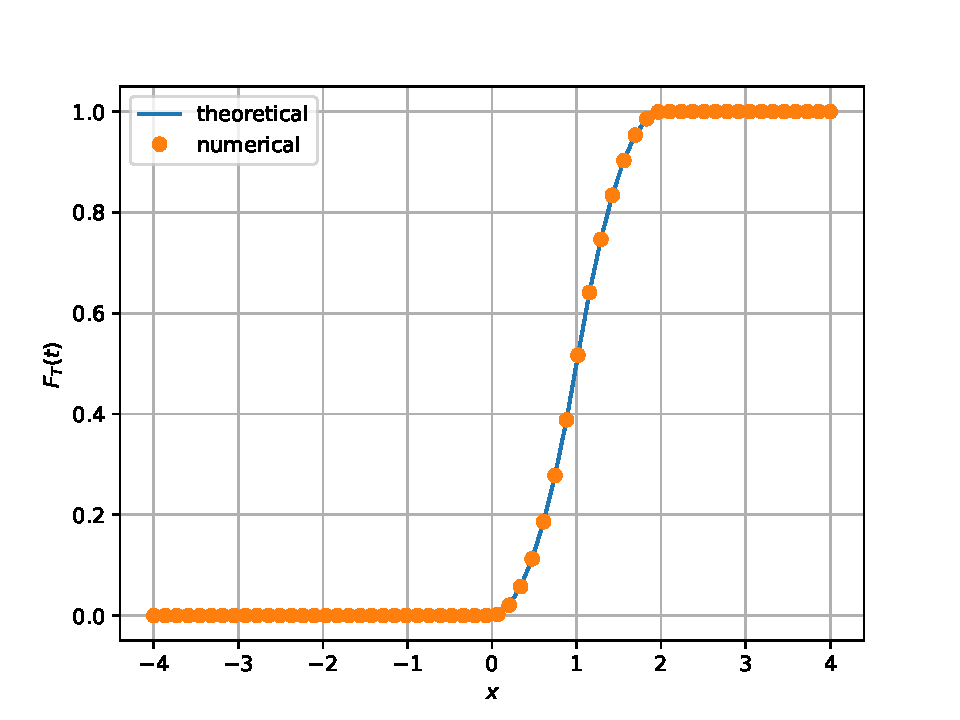
\includegraphics[scale = 0.6]{t_cdf.pdf}
    \caption{t-cdf}
    \label{fig:t-cdf}
\end{figure}

Take the code for pdf
\begin{lstlisting}
https://github.com/NareshBandaru13/Random-Numbers/blob/main/ex4/5/main2.py
\end{lstlisting}
Run in terminal
\begin{lstlisting}
python3 main2.py
\end{lstlisting}
\begin{figure}[H]
    \centering
    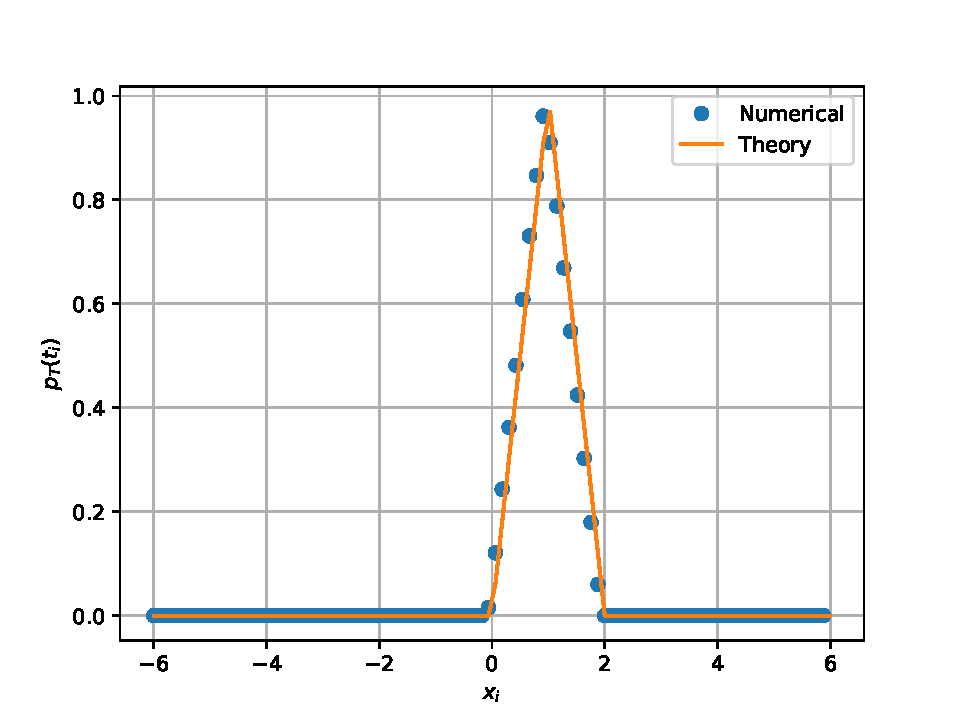
\includegraphics[scale = 0.6]{t.pdf}
    \caption{t-pdf}
    \label{fig:t-pdf}
\end{figure}

\end{enumerate}


\section{Maximul Likelihood}
\begin{enumerate}[label=\thesection.\arabic*
,ref=\thesection.\theenumi]

\item Generate 
\begin{equation}
Y = AX+N,
\end{equation}
where $A = 5 \text{ dB}, X \i \cbrak{1,-1}$\\
\solution
use bernouli function from exrand.c find the code
\begin{lstlisting}
https://github.com/NareshBandaru13/Random-Numbers/blob/main/ex5/1/exrand.c
\end{lstlisting}
run the terminal command
\begin{lstlisting}
gcc exrand.c -lm
./a.out
\end{lstlisting}


\item Generate 
\begin{equation}
Y = AX+N,
\end{equation}
where $A = 5$ dB,  and $N \sim N(0,1)$.
find the code
\begin{lstlisting}
https://github.com/NareshBandaru13/Random-Numbers/blob/main/ex5/2/main.py
\end{lstlisting}
run the command
\begin{lstlisting}
python3 main.py
\end{lstlisting}

\item Plot $Y$ using a scatter plot.
find the scatter plot\\
\solution
\begin{figure}[H]
    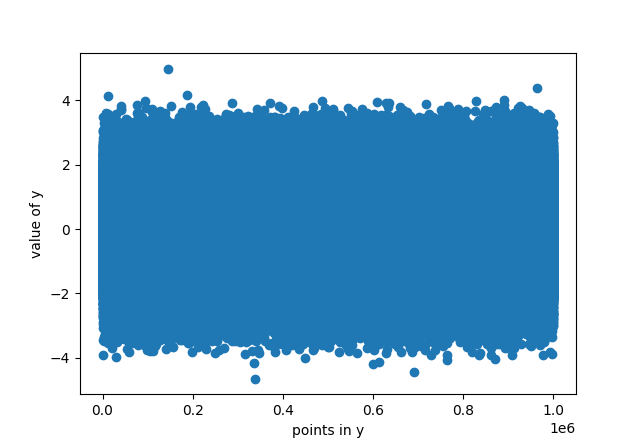
\includegraphics[scale = 0.6]{y.png}
    \caption{scatter plot}
    \label{fig:my_y}
\end{figure}

\item Guess how to estimate $X$ from $Y$.\\
\solution To estimate $X$ from $Y$, consider function:
\begin{align}
    \sgn(y) = 
    \begin{cases}
        -1, & y \in (-\infty,0] \\
        1, & y \in (0, \infty)
    \end{cases}
\end{align}
Using $\sgn{y}$, we can operate on $Y$ to find corresponding values of $X$.

\item
\label{ml-ch4_sim}
Find 
\begin{equation}
	P_{e|0} = \pr{\hat{X} = -1|X=1}
\end{equation}
and 
\begin{equation}
	P_{e|1} = \pr{\hat{X} = 1|X=-1}
\end{equation}

find the code below
\begin{lstlisting}
https://github.com/NareshBandaru13/Random-Numbers/blob/main/ex5/5/main.py
\end{lstlisting}
run the code
\begin{lstlisting}
python3 main.py
\end{lstlisting}
we get the values as 
$P_{(e|0)} = 0.310007$ \\
$P_{(e|1)} = 0.310142$ \\

\item Find $P_e$ assuming that $X$ has equiprobable symbols.

\solution
Assume a general value of $A$.\\
 Our estimation function predicts  the data above the $x$ axis correspond to $X=1$, and the data points below the $x$-axis correspond to $X=-1$.
We have:
\begin{align*}
    P_{e|0} &= \pr{\hat{X} = -1|X=1} \\
    &= \pr{AX+N<0|X=1} \\
    &= \pr{N<-A} \\
    &= \int_{-\infty} ^{-A} \frac{1}{\sqrt{2\pi}} e^{\frac{-x^2}{2}} dx \\
    &= \int_{A} ^{\infty} \frac{1}{\sqrt{2\pi}} e^{\frac{-x^2}{2}} dx \\
    &= Q_N(A)
\end{align*}
where $Q_N$ is the $Q$function of the normal distribution.
Similarly, 
\begin{align*}
    P_{e|1} &= \pr{\hat{X} = 1|X=-1} \\
    &= \pr{AX+N>0|X=-1} \\
    &= \pr{N>A} \\
    &= \int_{A} ^{\infty} \frac{1}{\sqrt{2\pi}} e^{\frac{-x^2}{2}} dx \\
    &= Q_N(A)
\end{align*}

Given X is equiprobable so we have
\begin{align*}
    P_e &= P_{e|0}  \pr{X=1} + P_{e|1}  \pr{X=-1} \\
    &= \frac{1}{2} P_{e|0} + \frac{1}{2} P_{e|1} \\
    &= \frac{1}{2} Q_N(A) + \frac{1}{2} Q_N(A) \\
    &= Q_N(A)
\end{align*}

\item
Verify by plotting  the theoretical $P_e$ with respect to $A$ from 0 to 10 dB.  
find the code below
\begin{lstlisting}
https://github.com/NareshBandaru13/Random-Numbers/blob/main/ex5/7/main.py
\end{lstlisting}
run the command
\begin{lstlisting}
python3 main.py
\end{lstlisting}
\begin{figure}[H]
    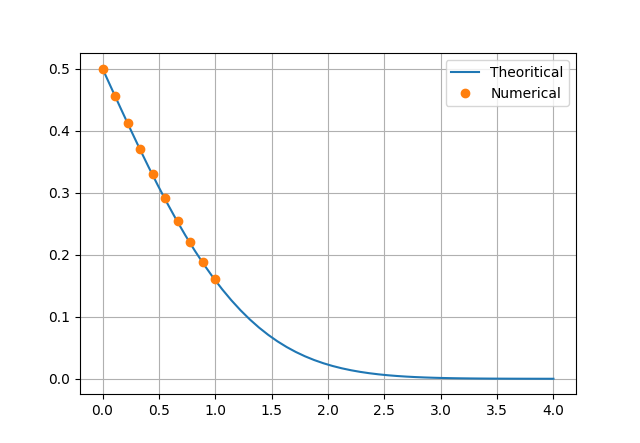
\includegraphics[scale = 0.6]{verifyp.png}
    \caption{verification of $p_e$}
    \label{fig:my_verifyP}
\end{figure}


\item Now, consider a threshold $\delta$  while estimating $X$ from $Y$. Find the value of $\delta$ that maximizes the theoretical $P_e$.

\solution
To estimate $X$ from $Y$, we consider
\begin{align*}
    X = 
    \begin{cases}
        1, & Y > \delta \\
        -1, & Y < \delta
    \end{cases}
\end{align*}
so we have
\begin{align*}
P_{e|0} &= \pr{\hat{X} = -1 | X = 1} \\
&= \pr{AX+N < \delta | X = 1} \\
&= \pr{N < \delta - A} \\
&= \int _{-\infty} ^{\delta - A} \frac{1}{\sqrt{2\pi}} e^{-\frac{x^2}{2}} dx \\
&= \int _{A - \delta} ^{\infty} \frac{1}{\sqrt{2\pi}} e^{-\frac{x^2}{2}} dx \\
&= Q_N(A - \delta) \\
\end{align*}

\begin{align*}
P_{e|1} &= \pr{\hat{X} = 1 | X = -1} \\
&= \pr{AX+N > \delta | X = -1} \\
&= \pr{N > \delta + A} \\
&= \int _{A - \delta} ^{\infty} \frac{1}{\sqrt{2\pi}} e^{-\frac{x^2}{2}} dx \\
&= Q_N(A + \delta) \\
P_e &= P_{e|0} \pr{X = 1} + P_{e|1} \pr{X = -1} \\
&= \frac{1}{2}(Q_N(A - \delta) + Q_N(A + \delta)) \\
\end{align*}

To minimise $P_e$,use differentiate wrt $\delta$:
\begin{align*}
 \frac{d}{d\delta} \left(\frac{1}{2}(Q_N(A - \delta) + Q_N(A + \delta))\right) &= 0\\
 \frac{1}{2} (\frac{1}{\sqrt{2\pi}} e^{-\frac{(\delta - A)^2}{2}} - \frac{1}{\sqrt{2\pi}} e^{-\frac{(A + \delta)^2}{2}} ) &= 0
\end{align*}
\begin{align*}
(\delta - A)^2 &= (\delta + A)^2& \\
\delta &= 0 
\end{align*}
so $\delta = 0$ maximize $P_e$

\item Repeat the above exercise when $p_{X}(0) = p$
\solution
we have:
\begin{align*}
    P_e &= P_{e|0} p+ P_{e|1} (1-p) \\
    &= p Q_N (A - \delta) + (1-p)Q_N (A + \delta) \\
\end{align*}
Differentiating wrt $\delta$ we get
\begin{align*}
p \frac{1}{\sqrt{2\pi}} e^{-\frac{(\delta - A)^2}{2}} - (1-p)\frac{1}{\sqrt{2\pi}} e^{-\frac{(A + \delta)^2}{2}} &= 0
\end{align*}
 Taking $\ln$ on both sides  and find $\delta$ :
 \begin{align*}
    \ln{p} - \frac{(\delta - A)^2}{2} &= \ln{(1-p)} - \frac{(\delta + A)^2}{2} \\
     \delta &= \frac{1}{2A} \ln{\frac{1-p}{p}}
 \end{align*}
if $p = \frac{1}{2}$ then $\delta = 0$ which verifies with above result.


\item Repeat the above exercise using the MAP criterion.

\solution
Assume that $\pr{X = -1} = p$, and $\pr{X = 1} = (1-p)$. Then, using the Law of Total Probability,
we have:
\begin{align*}
\nonumber p_Y(y) &= p_{Y|X = -1}(y|-1) \pr{X = -1} \\
&+ p_{Y| X = 1}(y|1) \pr{X = 1} \\
\nonumber &= p \times p_{(N - A)}(y) \\
&+ (1-p) \times p_{(N+A)} (y) 
\end{align*}
 
where $p_Y(y)$ is the pdf of $Y$. Now, $p_{(N-A)}$ is  the pdf of a shifted
normal distribution,so
\begin{align*}
    p_Y(y) &=  p \frac{e^{-\frac{(y+A)^2}{2}}}{\sqrt{2\pi}} + \left(1-p\right) \frac{e^{-\frac{(y-A)^2}{2}}}{\sqrt{2\pi}}
\end{align*}
MAP criterion,find $p_{X|Y}(x|y)$.  we use the Theorem of Conditional Probability:
\begin{align*}
    p_{X|Y}(x|y) &= \frac{p_{Y|X}(y|x) \times p_X(x)}{p_Y(y)}
\end{align*}
When $X=1$, we have:
\begin{align*}
    p_{X|Y}(1|y) &= \frac{p_{Y|X}(y|1) \times p_X(1)}{p_Y(y)} \\
    &= \frac{\left(1-p\right) \frac{e^{-\frac{(y-A)^2}{2}}}{\sqrt{2\pi}}}{ p \frac{e^{-\frac{(y+A)^2}{2}}}{\sqrt{2\pi}} + \left(1-p\right) \frac{e^{-\frac{(y-A)^2}{2}}}{\sqrt{2\pi}}} \\
    &= \frac{\left(1-p\right) e^{2yA}}{p + \left(1-p\right) e^{2yA}}
\end{align*}
Similarly, when $X = -1$, we have:
\begin{align*}
    p_{X|Y}(-1|y) &= \frac{p_{Y|X}(y|-1) \times p_X(-1)}{p_Y(y)} \\
    &= \frac{\left(p\right) \frac{e^{-\frac{(y+A)^2}{2}}}{\sqrt{2\pi}}}{ p \frac{e^{-\frac{(y+A)^2}{2}}}{\sqrt{2\pi}} + \left(1-p\right) \frac{e^{-\frac{(y-A)^2}{2}}}{\sqrt{2\pi}}} \\
   &= \frac{p}{p + \left(1-p\right) e^{2yA}} 
\end{align*}
    

Therefore, when $ p_{X|Y}(1|y) >  p_{X|Y}(-1|y)$, we have:
\begin{align*}
    \frac{\left(1-p\right) e^{2yA}}{p + \left(1-p\right) e^{2yA}} &> \frac{p}{p + \left(1-p\right) e^{2yA}} \\
    e^{2yA} &> \frac{p}{\left(1-p\right)} \\
    y &> \frac{1}{2A} \ln{\frac{p}{\left(1-p\right)}}
\end{align*}
Therefore, we can assert that $X = 1$, and $X = -1$ otherwise.
Now, consider when $p = \frac{1}{2} $.
We have:
\begin{align*}
    y &> \frac{1}{2A} \ln{\frac{p}{\left(1-p\right)}} \\
    &= \frac{1}{2A} \ln{1} \\
    &= 0
\end{align*}
Therefore, when $y > 0$, we choose $X = 1$, and we choose $X = -1$ otherwise.
\end{enumerate}

		
\section{Gaussian to Other}
\begin{enumerate}[label=\thesection.\arabic*
,ref=\thesection.\theenumi]
\item
Let $X_1 \sim  N(0,1)$ and $X_2 \sim N(0,1)$. Plot the CDF and PDF of \\
%
\begin{equation}
V = X_1^2 + X_2^2
\end{equation}
%
\solution The sum of squares of n independent standard random normal variables is  $\chi^2$ distribution with n degrees of freedom.\\
$$P_{\chi^{2}} (x|n)= \frac{x^{\frac{n}{2} -1} e^{\frac{-x}{2}}}{2^{\frac{n}{2}} \Gamma(
\frac{n}{2})} , \forall x\geq 0$$\\
Here k=2,

$$P_{\chi^{2}} (x|2) = P_{V}(v)= \frac{ e^{\frac{-v}{2}}}{2} $$
For the cummulative distribution
\begin{align*}
F_{V}(v)&=\int_{0}^{v} \frac{ e^{\frac{-v}{2}}}{2} dv\\
&=1-e^{\frac{-v}{2}}
\label{eq:eq6}
\end{align*}
To generate data for V , run the following code,
\begin{lstlisting}
https://github.com/NareshBandaru13/Random-Numbers/blob/main/ex6/1/coeffs.h
https://github.com/NareshBandaru13/Random-Numbers/blob/main/ex6/1/exrand.c
\end{lstlisting}
Run the below command in terminal,
\begin{lstlisting}
gcc exrand.c -lm
\end{lstlisting}
The PDF plot of the $\chi^{2} (2)$ can be obtained by running the code below,
\begin{lstlisting}
https://github.com/NareshBandaru13/Random-Numbers/blob/main/ex6/1/main1.py
\end{lstlisting}
Use the following command in the terminal to run the code
\begin{lstlisting}
python3 main1.py
\end{lstlisting}
\begin{figure}[H]
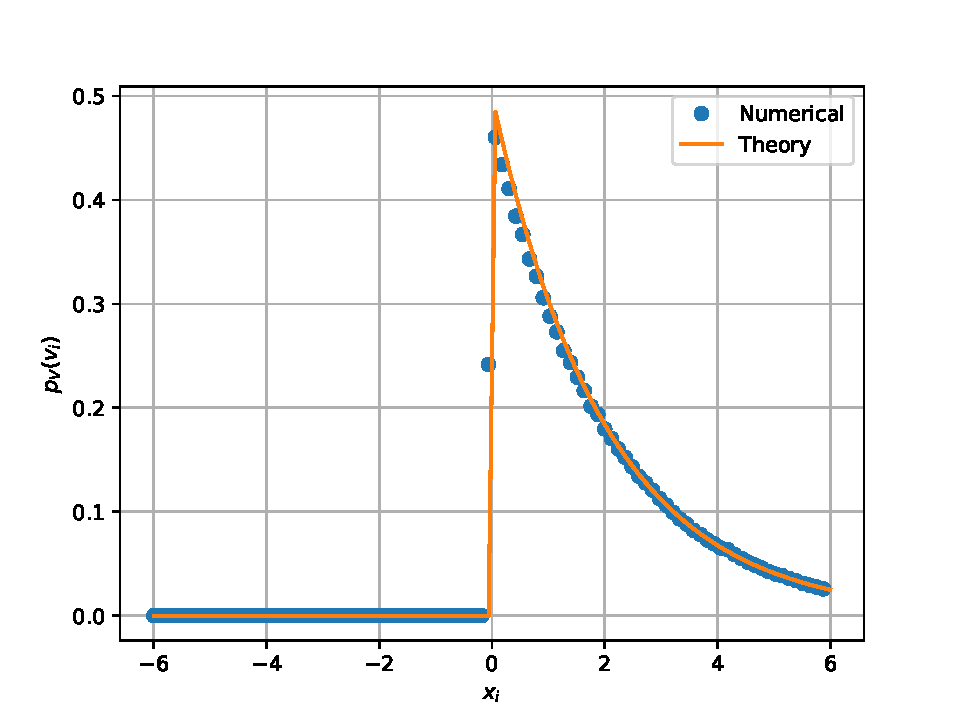
\includegraphics[width=0.5\textwidth]{v.pdf}
\caption{PDF plot}
\label{fig:chi_PDF}
\end{figure}
The CDF plot of the $\chi^{2} (2)$ can be obtained by running the code below,
\begin{lstlisting}
https://github.com/NareshBandaru13/Random-Numbers/blob/main/ex6/1/main2.py
\end{lstlisting}
Use the following command in the terminal to run the code
\begin{lstlisting}
python3 main2.py
\end{lstlisting}
\begin{figure}[H]
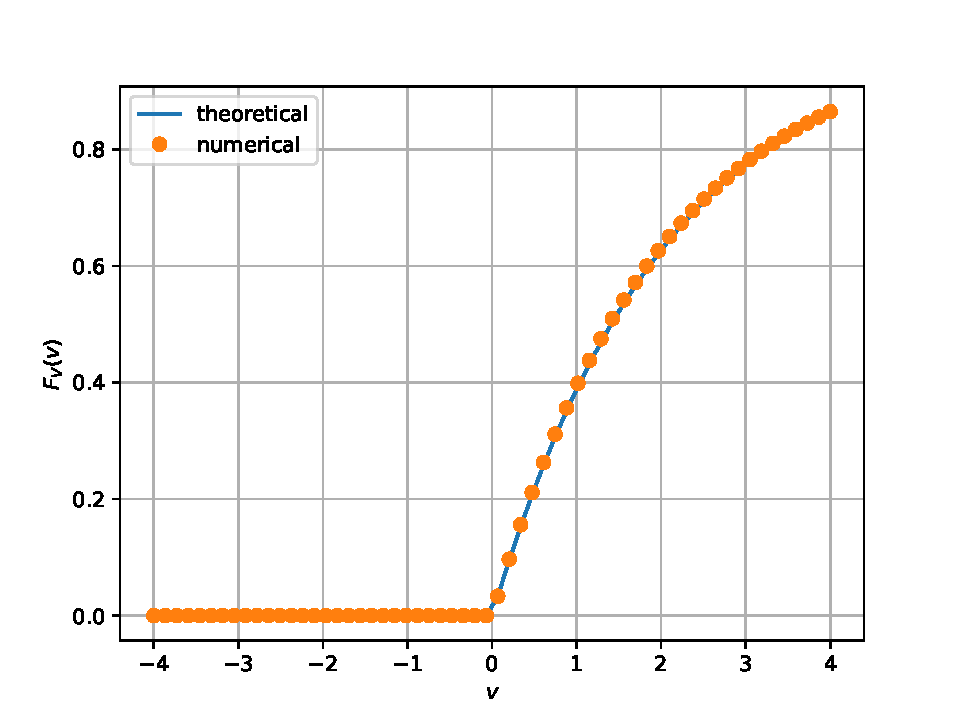
\includegraphics[width=0.5\textwidth]{v_cdf.pdf}
\caption{CDF plot}
\label{fig:chi_cdf}
\end{figure}



\item
If
\[
F_{V}(x) = 
\begin{cases}
1 - e^{-\alpha x} & x \geq 0 \\
0 & x < 0,
\end{cases}
\]
find $\alpha$.\\

\solution We will assume that $X_1$ and $X_2$ are i.i.d. 
Let
\begin{align*}
    X_1 = r \cos{\theta} \\
    X_2 = r \sin{\theta} 
\end{align*}
 The Jacobian Matrix is then defined as: 
 \begin{align*}
    J(r,\theta)  & = \myvec{\frac{\delta x_1}{\delta r}    & \frac{\delta x_1}{\delta \theta} \\ \frac{\delta x_2}{\delta r} & \frac{\delta x_2}{\delta \theta}}\\
    J &=  \myvec{\frac{\delta r \cos{\theta}}{\delta r} & \frac{\delta  r \cos{\theta}}{\delta \theta} \\ \frac{\delta r \sin{\theta}}{\delta r}  & \frac{\delta r \sin{\theta}}{\delta \theta}}\\
    J    & = \myvec{\cos\theta    & -R\sin\theta    \\ \sin\theta & R\cos\theta} \\
    |J(r,\theta)|  & = R
 \end{align*}
Then as $X_1$,$X_2$ are independent we have, 
\begin{align*}
    p_{X_1,X_2}(x_1,x_2) &= p_{X_1}(x_1)p_{X_2}(x_2) \\
    &= \frac{1}{2\pi} e^{\frac{-(x_1^2+x_2^2)}{2}} \\
    &= \frac{1}{2\pi} e^{\frac{-r^2}{2}}
\end{align*}
Now, since 
\begin{align*}
    p_{r, \theta}(r, \theta) &= |J(r,\theta)|p_{X_1, X_2}(x_1, x_2)      \\   
\intertext{we have:}     
p_{R, \theta}(r, \theta) & = \frac{r}{2\pi} e^{-\frac{r^2}{2}}  \\
p_R(r)&=\int_0^{2\pi} p_{R, \theta}(r, \theta) \\
   & = \int_0^{2\pi} \frac{r}{2\pi} e^{-\frac{r^2}{2}} d\theta   \\
    & = r e^{-\frac{r^2}{2}}  \\
    F_R(r) &= \pr{R \leq r} \\
    &= \int _{0} ^r f_R(r) dr \\
    &= 1 - e^{-\frac{r^2}{2}}
\end{align*}
$F_V(x)$ is given by:
\begin{align*}
    F_V(x) &= F_{X_1^2+X_2^2}(x) \\
    &= F_{R^2}{x} \\
    &= \pr{R^2 \leq x} \\
    &= \pr{R \leq \sqrt{x}} 
\end{align*}
Therefore, 
\begin{align*}
    F_V(x) = 
    \begin{cases}
        0 ,& x < 0 \\
        1 - e^{-\frac{x}{2}}, & x \geq  0\\
    \end{cases}
\end{align*}
by Comparing  we get $\alpha = \frac{1}{2}$ \\


\item Plot the CDF and PDf of
$$A = \sqrt{V}$$
\solution
To generate data for A , run the following code,
\begin{lstlisting}
https://github.com/NareshBandaru13/Random-Numbers/blob/main/ex6/3/coeffs.h
https://github.com/NareshBandaru13/Random-Numbers/blob/main/ex6/3/exrand.c
\end{lstlisting}
Run the below command in terminal,
\begin{lstlisting}
gcc exrand.c -lm
\end{lstlisting}
The PDF plot of A can be obtained by running the code below,
\begin{lstlisting}
https://github.com/NareshBandaru13/Random-Numbers/blob/main/ex6/3/main1.py
\end{lstlisting}
Use the following command in the terminal to run the code
\begin{lstlisting}
python3 main1.py
\end{lstlisting}

\begin{figure}[H]
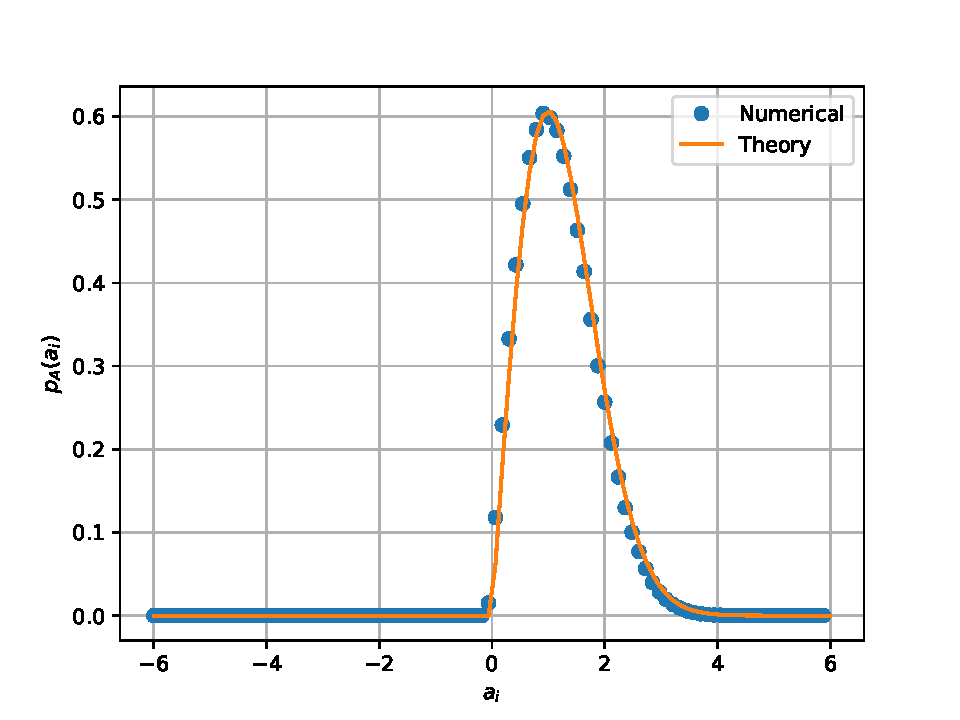
\includegraphics[width=0.5\textwidth]{a_pdf.pdf}
\caption{PDF}
\label{fig:A_PDF}
\end{figure}
The CDF plot of the A can be obtained by running the code below,
\begin{lstlisting}
https://github.com/NareshBandaru13/Random-Numbers/blob/main/ex6/3/main2.py
\end{lstlisting}
Use the following command in the terminal to run the code
\begin{lstlisting}
python3 main2.py
\end{lstlisting}
\begin{figure}[H]
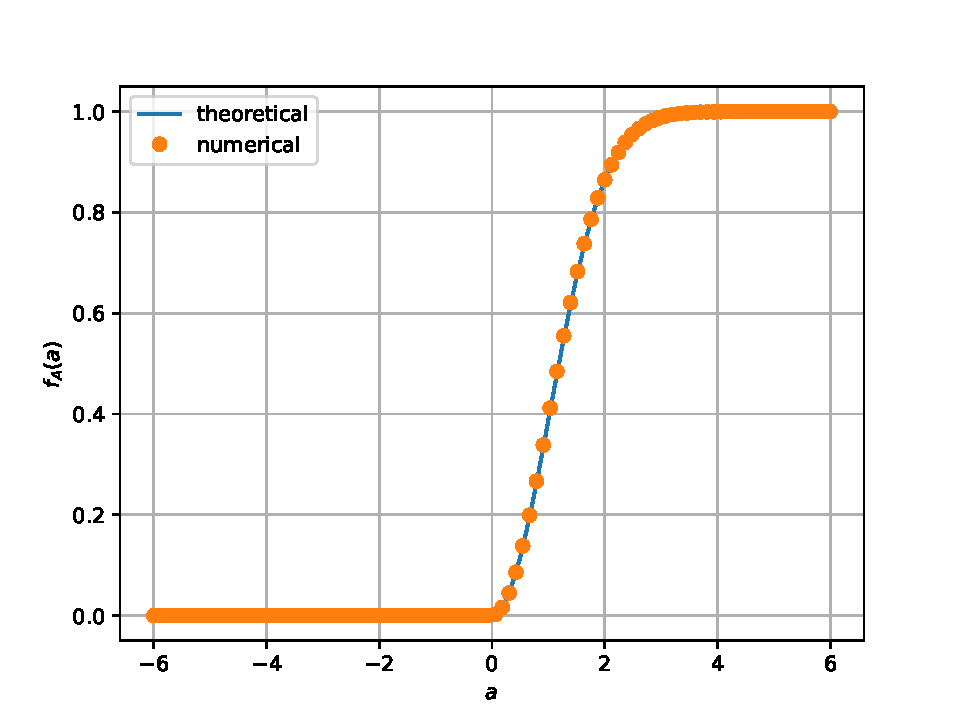
\includegraphics[width=0.5\textwidth]{a_cdf.pdf}
\caption{CDF}
\label{fig:A_cDF}
\end{figure}

	The CDF of $A$ for $x \ge 0$ is given by
	\begin{align*}
		F_A(x) &= \pr{A \le x} \\
		&= \pr{\sqrt{V} \le x} \\
		&= \pr{V \le x^2} \\
		&= F_V(x^2) \\
		&= 1 - \exp\brak{-\frac{x^2}{2}}
	\end{align*}
	
	The PDF of $A$ is given by
	\begin{align*}
		p_A(x) &= \frac{\der{}}{\der{x}} F_A(x) \\
		&= \frac{\der{}}{\der{x}} \brak{1 - \exp\brak{-\frac{x^2}{2}}} \\
		&= x \exp\brak{-\frac{x^2}{2}}
	\end{align*}
	
	Therefore,
	\begin{align*}
		F_A(x) &= 
		\begin{cases}
			1 - \exp\brak{-\dfrac{x^2}{2}} & x \geq 0 \\
			0 & \text{otherwise}
		\end{cases}	\\
		p_A(x) &= 
		\begin{cases}
			x \exp\brak{-\dfrac{x^2}{2}} & x \geq 0 \\
			0 & \text{otherwise}
		\end{cases}
	\end{align*}
\end{enumerate}

\end{document}